\makeatletter\let\ifGm@compatii\relax\makeatother
\documentclass[ucs,10pt]{beamer}
\mode<presentation>
%\hypersetup{pdfpagemode=FullScreen}

\usepackage{beamerthemesplit}
\usepackage{beamer_visser_um}
\usepackage{wrapfig}
\usepackage{hyperref}
%\usepackage{paralist}
%\usepackage[all]{xy}
%\usepackage{enumerate}
%\usepackage[ruled,vlined,lined,boxed,commentsnumbered]{algorithm2e}
%\usepackage{multirow}
%
%\usepackage[T1]{fontenc}
%\usepackage{listings}
%\usepackage{courier}
%\lstset{
%	 language=SPARQL,
%	 basicstyle=\footnotesize\ttfamily, % Standardschrift
%         %numbers=left,               % Ort der Zeilennummern
%         numberstyle=\tiny,          % Stil der Zeilennummern
%         %stepnumber=2,               % Abstand zwischen den Zeilennummern
%         numbersep=5pt,              % Abstand der Nummern zum Text
%         tabsize=2,                  % Groesse von Tabs
%         extendedchars=true,         %
%         breaklines=true,            % Zeilen werden Umgebrochen
%         keywordstyle=\color{blue},
%    		frame=single,         
% %        keywordstyle=[1]\textbf,    % Stil der Keywords
% %        keywordstyle=[2]\textbf,    %
% %        keywordstyle=[3]\textbf,    %
% %        keywordstyle=[4]\textbf,   \sqrt{\sqrt{}} %
%         stringstyle=\color{darkgreen}\ttfamily, % Farbe der String
%         showspaces=false,           % Leerzeichen anzeigen ?
%         showtabs=false,             % Tabs anzeigen ?
%         xleftmargin=10pt,
%         xrightmargin=10pt,
%         framexleftmargin=5pt,
%         framexrightmargin=5pt,
%         framexbottommargin=4pt,
%         backgroundcolor=\color{lightgray},
%         showstringspaces=false      % Leerzeichen in Strings anzeigen ?  
%}
%

\setlength{\unitlength}{\textwidth}  % measure in textwidths 


\title{Spectral Clustering for Axiom Selection}
%\title{Design of an engaging conversational agent for embedded systems}
\subtitle{}
\author{Zishi Wu}
\institute{Department of Computer Science\\ University of Miami \\
\vspace{.20cm}}
\date{\today}
\titlegraphic{\putat{-0.52}{-0.1}{
\includegraphics[height=1.5cm]{theUlogo}}}


\begin{document}

%%%%%%%%%%%%%%%%%%%%%%%%%%%%%%%%%%%%%%%%%%%%%%%%%%%%%%%%%%%%%

\frame{\titlepage}


\frame{
  \frametitle{Outline}    
  \tableofcontents
  \putat{0.40}{0.15}{
\includegraphics[width=.7\textwidth]{figures/intro}}
}

%%%%%%%%%%%%%%%%%%%%%%%%%%%%%%%%%%%%%%%%%%%%%%%%%%%%%%%%%%%%%

\section{Introduction}
\frame{
  \frametitle{Introduction}  
  \begin{block}{Definitions}
  	\begin{itemize}
  		\item What is Automated Theorem Proving (ATP)?
  		\item \textit{Logical formulae} are statements about a domain. 		
    	\item Show that the \textit{conjecture} is a 
    		\textit{logical consequence} of the axioms (a.k.a premises).	
		\item Applications:
			\begin{itemize}
				\item Formal verification of software - Compilers 
					(e.g. gcc, llvm)
				\item Formal verification of hardware - CPU 
					(e.g. 1994 Intel Pentium floating-point division bug)
				\item Interactive proof assistants for mathematics 
					(e.g. Isabelle, Mizar)
			\end{itemize}
  	\end{itemize}	
  \end{block}
}

%%%%%%%%%%%%%%%%%%%%%%%%%%%%%%%%%%%%%%%%%%%%%%%%%%%%%%%%%%%%%

\frame{
  \frametitle{Introduction}  
  \begin{block}{Example}
  	\begin{itemize}
		\item Axiom 1: \textit{All men are mortal}.
		\item Axiom 2: \textit{Socrates is a man}.
		\item Conjecture: \textit{Socrates is mortal}.
		\begin{figure}[H]
			\centering
			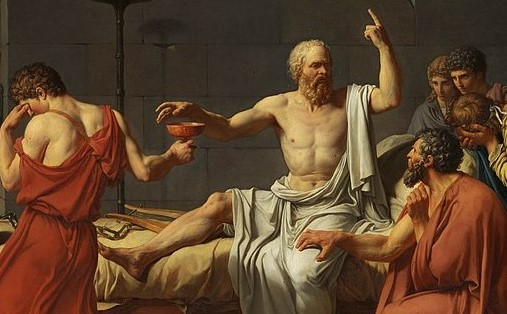
\includegraphics[scale=0.45]{figures/the-death-of-socrates.jpg}
  		\end{figure}  	
  	\end{itemize}	
  \end{block}
}


%%%%%%%%%%%%%%%%%%%%%%%%%%%%%%%%%%%%%%%%%%%%%%%%%%%%%%%%%%%%%

\frame{
  \frametitle{Logical Consequence}  
  \begin{block}{Logical Consequence}
  	\begin{itemize}
  		\item Every model of the axioms is a model of the conjecture.
  		\item A set of axioms has a \textit{model} if there is an 
  			\textit{interpretation} (assignment of boolean values) to the 
  			axioms such that the conjunction of the axioms evaluate to 
  			\textit{True}.
  		\item If we list all interpretations of $N$ formulae on a truth table, 
  			we get $2^{N}$ rows. This search space grows exponentially.
  		\item The faster way is to show that the union of the axioms and 
  			the negation of the conjecture is \textit{unsatisfiable}. 
  			$Ax \cup \neg C = \emptyset$
  		\item In other words, if no model of the axioms is a model of the
  			negated conjecture, then all models of the axioms are 
  			models of the conjecture.
  	\end{itemize}
  \end{block}
}

%%%%%%%%%%%%%%%%%%%%%%%%%%%%%%%%%%%%%%%%%%%%%%%%%%%%%%%%%%%%%

\frame{
  \frametitle{Problem Statement}  
  \begin{block}{Problem Statement}
  	\begin{itemize}
  		\item A \textit{large-theory} problem consists of a conjecture to be 
  			proven, and a large number of axioms to be considered.
  		\item However, the solution set(s) usually consist of a few axioms.
  		\item How do we select the necessary axioms? This is known as the 
  			problem of \textit{premise selection}.
  	\end{itemize}
  		
  	\begin{figure}[H]
		\centering
		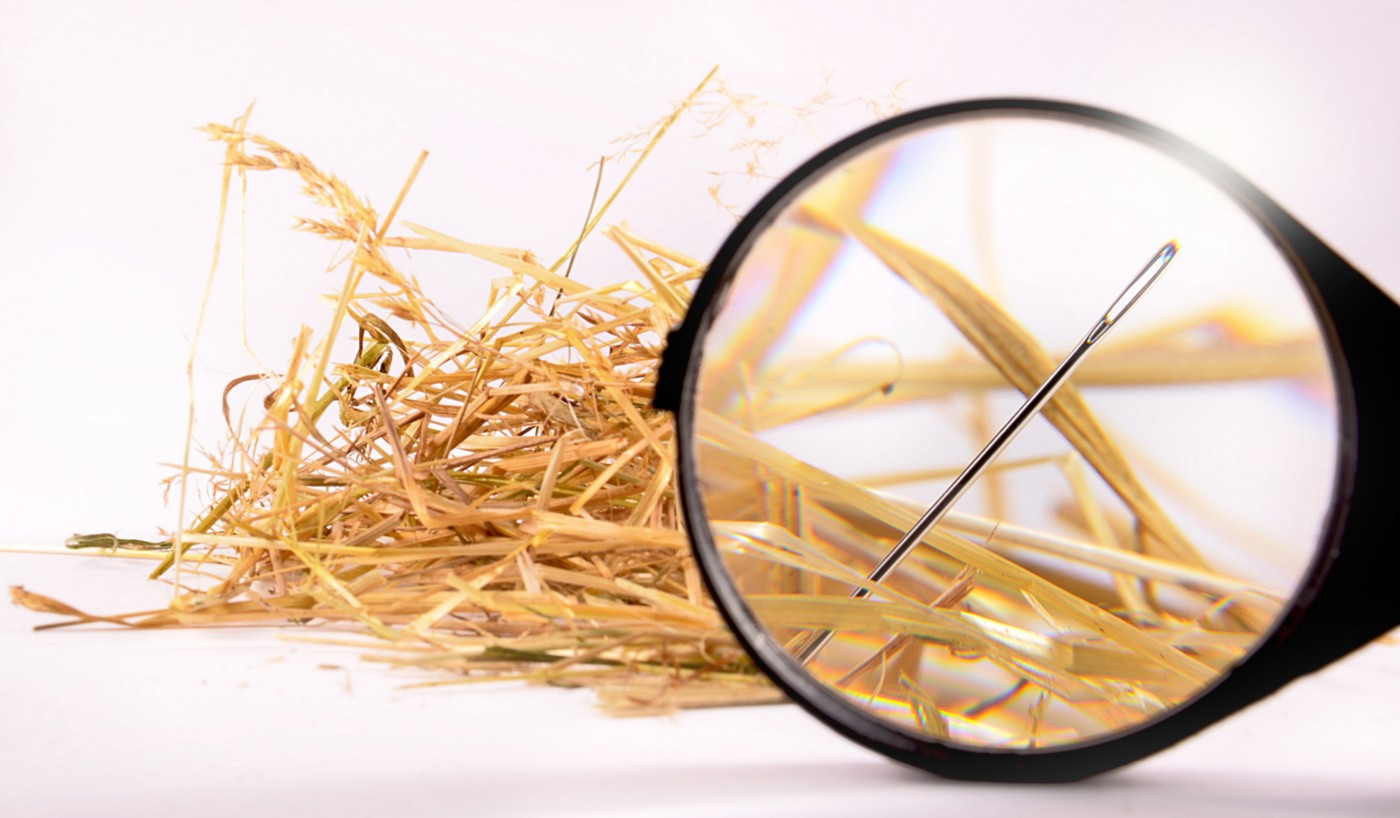
\includegraphics[scale=0.1]{figures/needle-in-haystack.jpeg}
  	\end{figure}
  \end{block}
}

%%%%%%%%%%%%%%%%%%%%%%%%%%%%%%%%%%%%%%%%%%%%%%%%%%%%%%%%%%%%%

\section{Related Work}
\frame{
  \frametitle{Benchmark Data}  
  \begin{block}{MPTP2078 Dataset}
  	\begin{itemize}
  	  	\item Thousands of Problems for Theorem Provers (TPTP) \cite{Sut17}
  		\begin{itemize}
			\item Standard set of test problems.	
  		\end{itemize}
  		\item Benchmark dataset of 2078 problems known as the 
  			Mizar Problems for Theorem Provers (MPTP2078) \cite{AH14}.
  			\begin{itemize}
  	  		\item Encodes problems from the Mizar Mathematical Library (MML) 	
  	  			of formalized mathematics into first-order logic form.
  			\end{itemize}
  		\item There are two versions of each problem:
  		\begin{itemize}
  			\item Bushy = smaller version (3 to 40 axioms, 1 to 15 needed)
  			\item Chainy = larger version (10 to 500 axioms, 2 to 119 needed)	
  		\end{itemize}
  	\item Premise selection performance compared to state-of-the-art 
  		Automated Theorem Provers: 
  		\begin{itemize}
  			\item E \cite{E-Sch13-LPAR}
  			\item Vampire \cite{Vampire-KV13}
  		\end{itemize}	
  	\end{itemize}	
  \end{block}
}

%%%%%%%%%%%%%%%%%%%%%%%%%%%%%%%%%%%%%%%%%%%%%%%%%%%%%%%%%%%%%

\frame{
  \frametitle{Ranking Problem}  
  \begin{block}{Ranking Problem}
  	\begin{itemize}
  		\item  Alama et al. \cite{AH14} formulated premise selection as a 
  			\textit{ranking problem}:
  			\begin{itemize}
  				\item Rank the axioms by how likely they are to prove a 
  					conjecture, based on some kind of user-defined 
  					similarity metric.
  				\item Choose a threshold value.
  				\item Select all axioms whose score is above that threshold.
  			\end{itemize}
  		\item Also a \textit{classification problem}: 
  			given a feature matrix consisting of the similarity values between 
  			formulae in a problem, train different machine learning methods on
  			the data to classify if an axiom is \textit{likely} or 
  			\textit{unlikely} to be in the proof.
  	\end{itemize}	
  \end{block}
}

%%%%%%%%%%%%%%%%%%%%%%%%%%%%%%%%%%%%%%%%%%%%%%%%%%%%%%%%%%%%%

\frame{
  \frametitle{Related Work}  
  \begin{block}{Extended Hutchinson Distance}
  	\begin{itemize}
  		\item To construct an adjacency matrix, we require a measure of 
  			similarity or dissimilarity between each pair of nodes in a graph.
  		\item Liu \cite{Liu2017Metric} proposed a dissimilarity metric 
  			between two terms $\Delta_{1}$ and $\Delta_{2}$, that extends 
  			the Hutchinson distance \cite{Hut97}.
  		\item Calculated by finding the Least Generalized Generalization 
  			(\textit{lgg}) between two formulae. A term $\Delta$ is the 
  			\textit{lgg} of $\Delta_{1}$ and $\Delta_{2}$ iff
  			\begin{itemize}
  				\item There are substitutions $\theta_{1}$ and $\theta_{2}$
  					such that $\Delta \theta_{1} = \Delta_{1}$ and 
  					$\Delta \theta_{2} = \Delta_{2}$.
  				\item There exists no term $\Delta'$ and substitutions
  					$\sigma$, $\sigma_{1}$ and $\sigma_{2}$ such that 
  					$\Delta \sigma_{1} = \Delta'$ and 
  					$\Delta \sigma_{2} = \Delta'$.
  			\end{itemize}
  	\end{itemize}	
  \end{block}
}

%%%%%%%%%%%%%%%%%%%%%%%%%%%%%%%%%%%%%%%%%%%%%%%%%%%%%%%%%%%%%

\frame{
  \frametitle{Related Work}  
  \begin{block}{Least Generalized Generalization Example}
  	\begin{itemize}
  	  	\item Note that the substitutions $\theta_{1}$ and $\theta_{2}$ are 
  	  		not limited to a single substitution rule. They can also consist  
  	  		of multiple substitution rules occurring one after the other.
  	\end{itemize}
  	\begin{figure}[H]
  		\centering
		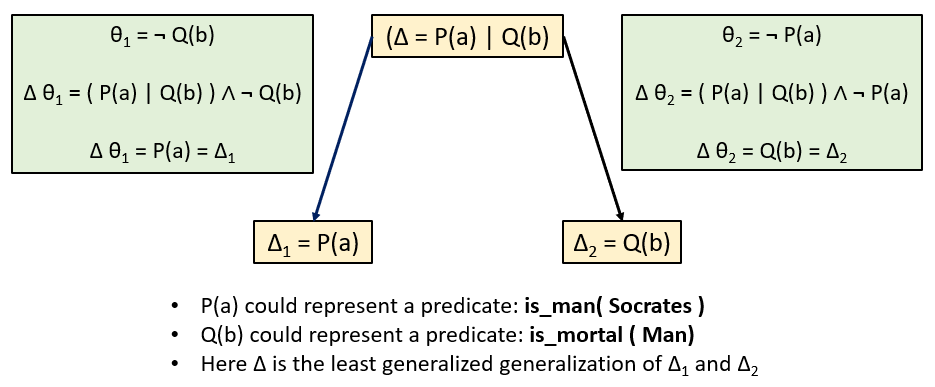
\includegraphics[scale=0.53]{figures/least-generalized-generalization-example.png}
  	\end{figure}
  \end{block}
}

%%%%%%%%%%%%%%%%%%%%%%%%%%%%%%%%%%%%%%%%%%%%%%%%%%%%%%%%%%%%%

\frame{
  \frametitle{Related Work}  
  \begin{block}{Extended Hutchinson Distance}
  	\begin{itemize}
  		\item If there is no Least Generalized Generalization $\Delta$
  			between two terms $\Delta_{1}$ and $\Delta_{2}$, then their 
  			extended Hutchinson distance is $\infty$. Formally,
  			\textit{dissimilarity}($\Delta_{1}$, $\Delta_{1}$) $= \infty$
  				iff $lgg(\Delta_{1}, \Delta_{2}) = \emptyset$.
  		\item If there exists a Least Generalized Generalization $\Delta$
  			between two terms $\Delta_{1}$ and $\Delta_{2}$, then the 
  			Extended Hutchinson Distance says:
  				\begin{itemize} 
  					\item More total substitutions required (from the 
  					\textit{lgg} to both terms) equates to a higher 
  						dissimilarity score.
  					\item Fewer total substitutions required equates to a 
  						lower dissimilarity score.
  				\end{itemize}
  		\item Note that this is a simplication of Qinghua's actual metric,
  			which is more complicated.
  		\item As expected, for any term $\Delta_{1}$,
			\textit{dissimilarity($\Delta_{1}$, $\Delta_{1})$} = 0
  	\end{itemize}	
  \end{block}
}

%%%%%%%%%%%%%%%%%%%%%%%%%%%%%%%%%%%%%%%%%%%%%%%%%%%%%%%%%%%%%
\section{Methodology}

\frame{
  \frametitle{Graph Matrices}  
  \begin{block}{Graph Laplacian Matrix}
  	\begin{itemize}
  		\item Von Luxburg \cite{vonLuxburg2007} describes this technique to 
  			cluster vertices in an undirected graph according to some 
  			user-defined similarity metric.
  		\item Adjacency matrix $A$ consists of edge weights between pairs 
  			of vertices that represent their similarity.
  		\item Degree matrix $D$ is a diagonal matrix where the $i^{th}$ 
  			element is the sum of the elements of the $i^{th}$ column of $A$.
  		\item Un-normalized Graph Laplacian matrix.
		\begin{itemize}
			\item $L = D\ –\ A$
		\end{itemize}
		\item Normalized Graph Laplacian matrix contains \textit{features}
			of the graph
		\begin{itemize}
			\item $L_{norm} = I\ –\ (D^{-1/2}\ L\ D^{-1/2})$
		\end{itemize}
  	\end{itemize}	
  \end{block}
}

%%%%%%%%%%%%%%%%%%%%%%%%%%%%%%%%%%%%%%%%%%%%%%%%%%%%%%%%%%%%%

\frame{
  \frametitle{Example Graph}  
  \begin{block}{Calculate Normalized Laplacian Matrix}
  	\begin{itemize}
  		\item Adjacency, Degree, and Un-normalized Graph Laplacian
  		\[ 
  		A = \begin{bmatrix}
		0 & 3 & 0 \\
		3 & 0 & 1 \\
		0 & 1 & 0
		\end{bmatrix} 
		\quad
		D = \begin{bmatrix}
		3 & 0 & 0 \\
		0 & 4 & 0 \\
		0 & 0 & 1
		\end{bmatrix}
		\quad
		L = \begin{bmatrix}
		0 & 3 & 0 \\
		3 & 0 & 1 \\
		0 & 1 & 0
		\end{bmatrix}
		\]
		\item Normalized Graph Laplacian
		\[ 
  		L_{norm} = \begin{bmatrix}
		1 & 0 & 0 \\
		0 & 1 & 0 \\
		0 & 0 & 1
		\end{bmatrix} -
		\begin{bmatrix}
		\dfrac{1}{\sqrt{3}} & 0 & 0 \\
		0 & 1/2 & 0 \\
		0 & 0 & 1
		\end{bmatrix} 
		\begin{bmatrix}
		0 & 3 & 0 \\
		3 & 0 & 1 \\
		0 & 1 & 0
		\end{bmatrix}
		\begin{bmatrix}
		\dfrac{1}{\sqrt{3}} & 0 & 0 \\
		0 & 1/2 & 0 \\
		0 & 0 & 1
		\end{bmatrix} 
		\]
  	\end{itemize}	
  \end{block}
}

%%%%%%%%%%%%%%%%%%%%%%%%%%%%%%%%%%%%%%%%%%%%%%%%%%%%%%%%%%%%%

\frame{
  \frametitle{Methodology}  
  \begin{block}{Graph Representation}
  	\begin{itemize}
  		\item Used Extended Hutchinson distance to get dissimilarity values 
  			of all pairs of vertices in a problem.
  		\item Let $\Phi_1$ and $\Phi_1$ represent two formulae with 
  		dissimilarity of $dsim(\phi_i,\phi_j)$. We convert dissimilarity 
  		values into similarity values using the following formula:
  			\begin{itemize}
  				\item $maxdsim(\mathcal{F}) = max_{\phi_i,\phi_j \in \mathcal{F}} (dsim(\phi_i,\phi_j) \neq \infty)$
  				\item $sim(\Phi_1,\Phi_2,\mathcal{F}) = \textrm{max}(0, maxdsim(\mathcal{F}) - dsim(\Phi_1,\Phi_2))$
  			\end{itemize}
  		\item The logic problem becomes a fully-connected and undirected graph
  		\begin{itemize}
  			\item Vertices $V$ = $\{$Axioms $\cup$ Conjecture$\}$
  			\item Edges $E$ = similarity values between vertices  		
  		\end{itemize}
  	\end{itemize}	
  \end{block}
}

%%%%%%%%%%%%%%%%%%%%%%%%%%%%%%%%%%%%%%%%%%%%%%%%%%%%%%%%%%%%%

\frame{
  \frametitle{Spectral Clustering Algorithm}  
  \begin{block}{Spectral Clustering}
  	\begin{itemize}
  		\item A Tutorial on Spectral Clustering \cite{vonLuxburg2007}
  		\begin{enumerate}
    		\item Construct a weight matrix W (i.e. adjacency matrix A) 
    		containing similarity values of the edges of the graph.
  			\item Compute the normalized Laplacian matrix $L_{norm}$ from $W$.
			\item Compute the first $k$ eigenvectors $v_{1}, ..., v_{k}$ of 
				$L_{norm}$ and construct a feature matrix $U$ from those 
				eigenvectors.
			\item For $i = 1, ..., n$, let $p_{i}$ be the feature vector for 
				the $i^{th}$ vertex, corresponding to the $i^{th}$ row of $U$.
			\item Cluster the vertices based on their feature vectors into 
				$k$ clusters: $C_{1}, C_{2}, ..., C_{k}$. Denote the cluster 
				containing the conjecture as $C_{C}$.
  		\end{enumerate}
  		
  		\item A problem may have more than one set of solutions, but the 
	  		conjecture cluster needs only to contain the axioms for one 
	  		solution to be deemed a successful clustering.
  	\end{itemize}
  \end{block}
}

%%%%%%%%%%%%%%%%%%%%%%%%%%%%%%%%%%%%%%%%%%%%%%%%%%%%%%%%%%%%%

\frame{
  \frametitle{K-Means Clustering}  
  \begin{block}{K-Means Clustering Problems}
  	\begin{enumerate}[5]
    	\item Cluster the vertices based on their feature vectors into $k$ 
    		clusters: $C_{1}, C_{2}, ..., C_{k}$.
  		\begin{itemize}
  			\item Each run of k-means chooses a different set of initial 
  				centroids for the $k$ clusters.
			\item Results in different clusterings each run.
  		\end{itemize}
  	\end{enumerate}
  	\begin{itemize}
  	  	\item We need a deterministic way of clustering that doesn’t 
			change over multiple runs of k-means.
		\item We also need to figure out the optimal value for the parameter 
			$k$, the number of clusters.
  	\end{itemize}
  \end{block}
}

%%%%%%%%%%%%%%%%%%%%%%%%%%%%%%%%%%%%%%%%%%%%%%%%%%%%%%%%%%%%%

\frame{
  \frametitle{K-Means Clustering}  
  \begin{block}{Solution to Initial Centroids Problem}
  	\begin{itemize}
    	\item Solution description here.
  	\end{itemize}
  \end{block}
}

%%%%%%%%%%%%%%%%%%%%%%%%%%%%%%%%%%%%%%%%%%%%%%%%%%%%%%%%%%%%%

\frame{
  \frametitle{K-Means Clustering}  
  \begin{block}{Solution to Number of Clusters Problem}
  	\begin{itemize}
    	\item Solution description here.
  	\end{itemize}
  \end{block}
}

%%%%%%%%%%%%%%%%%%%%%%%%%%%%%%%%%%%%%%%%%%%%%%%%%%%%%%%%%%%%%

\frame{
  \frametitle{Prediction of Optimal Number of Clusters}  
  \begin{block}{Median Regression}
  	\begin{itemize}
    	\item Method description here.
  	\end{itemize}
  \end{block}
}

%%%%%%%%%%%%%%%%%%%%%%%%%%%%%%%%%%%%%%%%%%%%%%%%%%%%%%%%%%%%%

\frame{
  \frametitle{Evaluation Metrics}  
  \begin{block}{Evaluation Metrics}
  	\begin{itemize}
    	\item Selectivity
    	\item Precision Score
    	\item Adequacy
  	\end{itemize}
  \end{block}
}

%%%%%%%%%%%%%%%%%%%%%%%%%%%%%%%%%%%%%%%%%%%%%%%%%%%%%%%%%%%%%
\section{Results}

\frame{
  \frametitle{Results}  
  \begin{block}{Predicted Number of Clusters}
  	\begin{itemize}
    	\item Result description here.
  	\end{itemize}
  \end{block}
}

%%%%%%%%%%%%%%%%%%%%%%%%%%%%%%%%%%%%%%%%%%%%%%%%%%%%%%%%%%%%%
\section{Results}

\frame{
  \frametitle{Results}  
  \begin{block}{Evaluation on Bushy and Chainy Problems}
  	\begin{itemize}
    	\item Result description here.
  	\end{itemize}
  \end{block}
}

%%%%%%%%%%%%%%%%%%%%%%%%%%%%%%%%%%%%%%%%%%%%%%%%%%%%%%%%%%%%%
\section{Conclusion}

\frame{
  \frametitle{Conclusion}  
  \begin{block}{Conclusion}
  	\begin{itemize}
    	\item Spectral clustering method extensions.
    	\item Dissimilarity method extensions.
    	\item Mention paper submitted to conference name.
    	\item Thanks to Qinghua Liu, Zihao Wang, and Dr. Geoff Sutcliffe.
  	\end{itemize}
  \end{block}
}

%%%%%%%%%%%%%%%%%%%%%%%%%%%%%%%%%%%%%%%%%%%%%%%%%%%%%%%%%%%%%

\bibliographystyle{alpha}
\bibliography{references}
\end{document}